\documentclass[times, utf8, diplomski, numeric]{fer}
\usepackage{booktabs}

\usepackage{float} % "place table exactly here" package

\begin{document}

\thesisnumber{1954}

\title{Stvarnovremensko praćenje parametara ispravnosti rada u sustavu za raspodijeljenu obradu tokova podataka}

\author{Mislav Jakšić}

\maketitle

\izvornik

\zahvala{Hvala svima!}

\tableofcontents

\chapter{Uvod}

Raspodijeljeni sustavi su nepouzdani. Pogreška u sklopovlju, operacijskom sustavu, programu ili mreži može izazvati ispad bilo kojeg dijela sustava. Ispadi u raspodijeljenom sustavu mogu pokrenuti lanac ispada. Ako ispad ne uzrokuje lanac ispada sustav će i dalje patiti jer će program i dalje zahtijevati računalno vrijeme i memoriju, a s njima neće obavljati koristan posao. U najgorem slučaju ispad može izazvati potpuno zatajenje sustava gdje je jedini lijek iznova pokrenuti sve njegove dijelove. U najboljem slučaju ispad će samo smanjiti učinkovitost sustava. Bez pažljivog nadzora raspodijeljenog sustava teško je otkriti ispad, a još teze otkloniti izvor ispada.

Zadatak nadzora je otkriti ispad i njegov uzrok. \citep{rassus-manual} ispade dijeli na ispad procesa, pogreške u komunikaciji, vremenske pogreške, pogrešan odgovor i bizantske pogreške. Ako se ispad želi otkriti potrebno je pratiti vrijednosti koje ukazuju da se ispad dogodio. Korisne vrijednosti mogu biti zauzeće memorije, brzina obrade zahtjeva, sadržaj poruke ili duljina uspostave komunikacijskog kanala. Nadzirani program vrijednosti predaje nadzorniku koji je čovjek ili program. Ako nadzor obavlja program on treba biti pouzdaniji od nadziranog programa inače je problem nadzora udvostručen, a ne riješen.

Prvi korak u izradi pouzdanog sustava nadzora je izrada pouzdanog sakupljača vrijednosti. Prije same izrade istražene su ideje, sukobljene su arhitekture i uspoređena postojeća rješenja. Kako bi naglasak na idejama, arhitekturama i izradi rješenja bio podjednak napravljen je sakupljač za jedan raspodijeljeni sustav. Kada bi umjesto njega bio napravljen svestran sakupljač koji može sakupljati vrijednosti raznolikog sklopovlja, operacijskih sustava i programa misli o arhitekturi bile bi izražene na uštrp onima o izradi programa. Nadzirani sustav je Apache Kafka, popularni sustav za raspodijeljenu obradu tokova podataka.

\chapter{Sustavi za raspodijeljenu obradu tokova podataka}

\citep{ilprints535} razlikuje tok podataka od skupa podataka. Toku podaci dolaze stalno, u nepoznatom redoslijedu, bez znaka kada će prestat i bit će odbačeni nakon što su pročitani. Ovi sustavi su raspodijeljeni jer se tok mora obraditi brzo. Primjer problema toka podatka su kartično plaćanje, praćenje korisnika mrežnih stranica, posluživanje reklama i preporuka. Svi navedeni problemi imaju mnogo izvora i ponora podataka. Kako sakupiti, zabilježiti, te dostaviti podatke na ponor gdje će se obraditi su problemi za koje sustavi za raspodijeljenu obradu tokova podataka nude rješenje. Zato što su tokovi podatka raznovrsni razvijeno je mnoštvo alata za njihovu obradu. Alate razlikujemo po načinu sakupljanja podataka, po mogućnostima toka, po arhitekturi i načinu zapisivanja podataka.

Prije razvoja sakupljača vrijednosti potrebno je usporediti i izabrati alat za raspodijeljenu obradu podataka. Kako bi usporedba alata i izvedba sakupljača bila jednostavnija u obzir su uzeti samo javno dostupni alati. Većina takvih alata koristi model objavi/pretplati. Umjesto da se usporede svi javno dostupni alati izabran je predstavnik iz svakog važnog skupa alata:
\begin{itemize}
    \item Apache Kafka je predstavnik popularnih alata za raspodijeljenu obradu tokova podataka
    \item Apache Pulsar je predstavnik modernih alata. \citep{yahoo-blogpost} je 2016. objavio Pulsar dok je \citep{kafka-whitepaper} objavio Kafku 2011. godine
    \item RabbitMQ je predstavnik alat koji potiskuju podatke prema korisnicima. Za razliku od RabbitMQ korisnici Kafke i Pulsara moraju povlačiti podatke
\end{itemize}

\section{Model objavi/pretplati}

\begin{figure}[H]
    \centering
    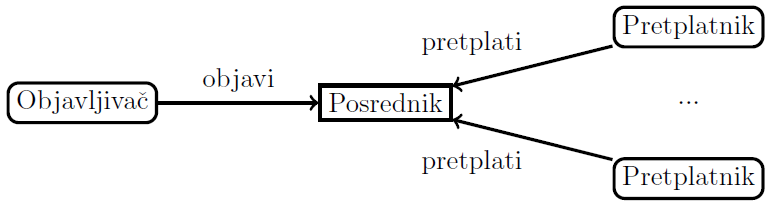
\includegraphics[width=0.8\textwidth]{PublishSubscribe.png}
    \caption{Model objavi/pretplati}
    \label{fig:publish-subscribe}
\end{figure}

Apache Kafka, Apache Pulsar i RabbitMQ koriste model objavi/pretplati za razmjenu podataka između procesa. \ref{fig:publish-subscribe} prikazuje nužne dijelove modela objavi/pretplati. \citep{rassus-manual} navodi da se model objavi/pretplati sastoji od objavljivača koji šalju poruke, pretplatnika koji čitaju poruke i posrednika koji razmjenjuje poruke između njih. Posrednik zapisuje objavljene poruke i dopušta pretplatnicima da ih čitaju. Prednost modela objavi/pretplati nad izravnim razgovorom među procesima je što objavljivači i pretplatnici ne trebaju znati jedan za drugoga.

\section{Apache Kafka}

\begin{figure}[H]
    \centering
    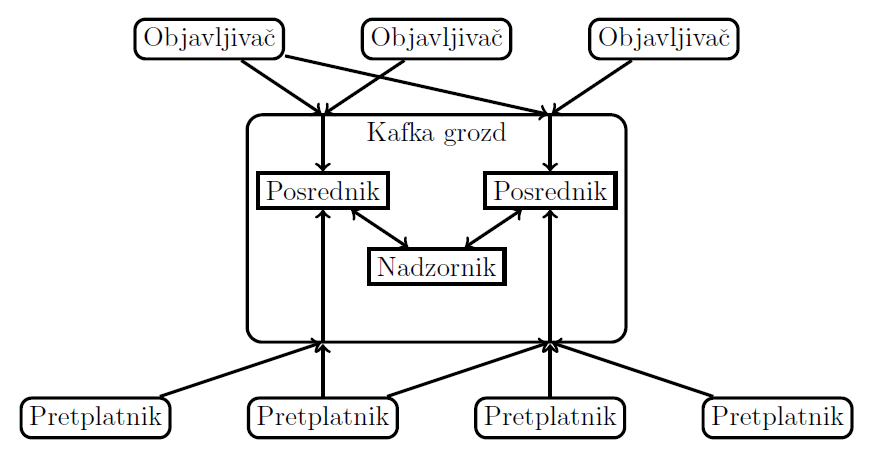
\includegraphics[width=0.8\textwidth]{KafkaCluster.png}
    \caption{Apache Kafka grozd}
    \label{fig:kafka-cluster}
\end{figure}

Apache Kafka je popularni alat za raspodijeljenu obradu tokova podataka. \ref{fig:kafka-cluster} prikazuje Kafka grozd. Svaki grozd sastoji se od ZooKeeper nadzornika i barem jednog posrednika. Nadzornik usklađuje posrednike. Objavljivači šalju poruke u temu grozda. Posrednici zapisuju poruke u pretinac teme. Pretplatnici čitaju poruke iz teme grozda i obrađuju podatke. \citep{kafka-whitepaper} \citep{kafka-docs} opisuju primjenu, arhitekturu i izvedbu Kafka pretplatnika, pretinca, posrednika, teme i objavljivača.

\subsection{Objavljivač}
Objavljivač je korisnički program koji šalje poruke u temu grozda. Poruka se nužno sastoji od sadržaja, teme na koju se objavljuje, oznake pretinca, odmaka u pretincu i vremena objave. Poruke se šalju u skupini nakon sto prođe određeno vrijeme ili se nakupi dovoljno poruka. \cite{kafka-compression} navodi kako poruke sažeti prije slanja. Tema je podijeljena na pretince. Pretinac je dnevnik u koji posrednik zapisuje poruke. Posrednik je poslužitelj koji zapisuje poruke u pretinac. Objavljivač ili ključem izabere pretinac u koji želi zapisati poruke ili se poruke šalju u svaki pretinac jednoliko. Posrednik će poslati potvrdu kada se poruke zapišu u pretinac vođe i izabrani broj usklađenih sljedbenika. Prije slanja sljedećeg skupa poruka objavljivač može pričekati potvrdu posrednika.

Ako se dogodi ispad objavljivača ili posrednika, objavljivač će ponovno poslati poruke. Objavljene poruke biti će dostavljene posredniku barem jednom. Ako je uvišestručavanje poruka nedopustivo, objavljivač može koristiti transakcijski način rada.

\subsection{Tema}
Tema je tok poruka, apstraktna umotvorina u koju objavljivači šalju poruke, a iz koje pretplatnici čitaju poruke. Posrednici se brinu da poruke budu zapisane. Biti pretplaćen na temu znači napraviti podtok poruka. Poruke objavljene u temu se ravnomjerno raspoređuju u podtokove. Svaki podtok ima pokazivač kojim pretplatnik čita poruke. Ako pokazivač dođe do kraja podtoka, pretplatnik se blokira dok se ne objavi nova poruka. Količina nepročitanih poruka u temi ne utječe na protok poruka kroz temu. Poruke u temi se brišu tek nakon određenog vremena. Tema je podijeljena na pretince s kojih posrednici čitaju i u koje pišu poruke. Kako bi poruke u pretincu bile dostupne nakon ispad posrednika, pretinac je moguće umnožiti.

\subsection{Posrednik}
Posrednik je poslužiteljski program koji zapisuje poruke objavljivača i poslužuje poruke pretplatnicima. Svaki posrednik dio je samo jednog Kafka grozda. Posrednici koriste Apache ZooKeeper za izvršavanje sporazumnog algoritma, pamćenje tema, njihovih pretinaca i usklađenih posrednika. Posrednik će poruke zapisati u pretinac onim redoslijedom kojim je objavljivač poslao poruke, ne redoslijedom kojim je posrednik primio poruke. Pretplatnici će s posrednika čitati poruke onim redoslijedom kojim su zapisane u pretinac.

Kada objavljivač objavi poruke na temu posrednik će zapisati poruke u određeni pretinac. Posrednik koristi sustav straničenja i tvrdi disk za zapisivanje poruka opisano u \cite{kafka-paging}. Umjesto da posrednik koristi memoriju procesa za priručnu memoriju posrednik poruke predaje sustavu straničenja operacijskog sustava. Operacijski sustav će poruke zapisati u stranice i pohraniti u nedodijeljene dijelove radne memorije. Poruke se zapisuju na tvrdi disk samo kada operacijski sustav želi osloboditi memoriju sustava straničenja. Opisano gospodarenje memorijom dopusta posredniku da čuva veliku količinu poruka bez gubitka učinkovitosti.

Pretplatnici često dohvaćaju uzastopne poruke pa se one čitaju iz priručne memorije umjesto iz tvrdog diska. Zahvaljujući sustavu straničenja priručna memorija sa zapisanim porukama će postojati neko vrijeme nakon ispada posrednika. Korištenjem sustava straničenja za zapisivanje poruka izbjegava se korištenje sakupljača smeća Java virtualnog stroja. Umjesto da se poruke zapisu dva puta, jednom u dodijeljenu memoriju procesa i jednom u sustav straničenja poruke se zapisu samo jednom u sustav straničenja.

Kada pretplatnik želi pročitati poruke posrednik će pronaći, pročitati i poslati poruke pretplatniku. \cite{linux-sendfile} \cite{java-zero-copy} opisuju kako posrednik s sendfile i zero-copy funkcijama čita poruke iz radne memorije i šalje u memoriju mrežne kartice u jednom koraku. Kako bi se dodatno ubrzao rad posrednici, objavljivači i pretplatnici grupe poruka čitaju, zapisuju i šalju u istom binarnom obliku. Prije slanja poruka pretplatnicima posrednik može sažeti poruke.

\subsection{Pretinac}

\begin{figure}[H]
    \centering
    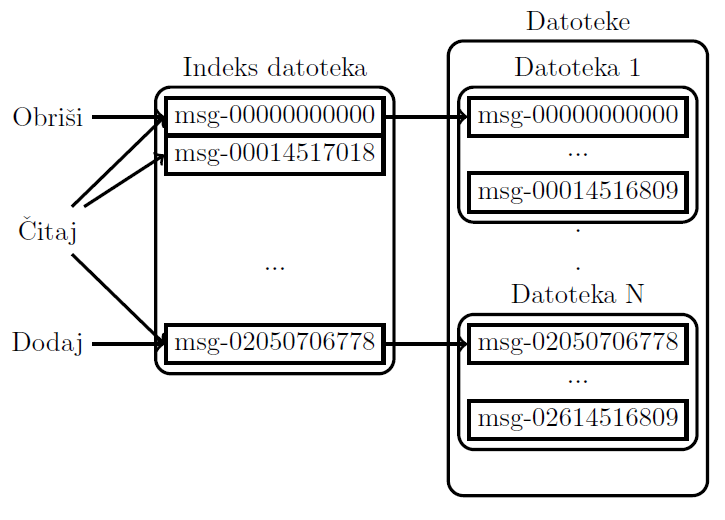
\includegraphics[width=0.8\textwidth]{KafkaLog.png}
    \caption{Kafka dnevnik}
    \label{fig:kafka-log}
\end{figure}

Pretinac je logički dnevnik i najmanja gradivna jedinica teme. Kada objavljivač objavi poruku u temu grozda posrednik poruke zapiše u pretinac teme. \ref{fig:kafka-log} prikazuje dnevnik izveden kao skup datoteka iste veličine. Kada posrednik zapiše poruke u pretinac on doda poruke na kraj datoteke. Datoteke se predaju sustavu straničenja operacijskog sustava tek nakon određenog vremena ili broja dodavanja. Svaka poruka ima jedinstvenu oznaku koja je ujedno i odmak unutar datoteke. Odmak sljedeće poruke računa se kao zbroj odmaka i veličine ranije poruke. Zato su oznake poruka jedinstvene i strogo rastuće ali nisu uzastopne.

Protok poruka kroz temu može biti toliki da izazove preopterećenje posrednika. Zato je temu moguće podijeliti na više pretinaca. Ako je B broj posrednika u Kafka grozdu onda tema može biti podijeljena na najviše B pretinaca. Svaki pretinac teme mora biti dodijeljen različitom posredniku.

Ako se dogodi ispad posrednika, poruke u pretincu postat će nedostupne. Ako poruke moraju biti dostupne čak i tijekom ispada posrednika pretinac se mora umnožiti. Svaki pretinac može biti umnožen najviše B puta ako je B broj posrednika u Kafka grozdu. Svaki umnoženi pretinac bit će dodijeljen različitom posredniku jer dodjela istom ne povećava dostupnost uslijed ispada. Ako se pretinac umnoži B puta onda će poruke u pretincu postati nedostupne tek ako se dogodi strogo vise od B-1 ispada posrednika.

Kada su pretinci umnoženi potrebno je ujednačiti poruke u svakom umnoženom pretincu. Zato će jedan posrednik biti vođa pretinca, a ostali posrednici će biti pratitelji pretinca. Svaki posrednik može biti vođa najviše jednog pretinca po temi. Vođa pretinca je jedini posrednik koji smije čitati ili pisati poruke u pretinac. Zadaća pratitelja je preusmjeriti korisnike na vođu pretinca i uskladiti svoj pretinac s pretincem vođe. Pratitelji mogu preusmjeriti korisnike na vođu pretinca tako da pitaju ZooKeepera tko je vođa kojeg pretinca. Svaki pratitelj ima pretplatnika koji čita poruke iz pretinca vođe i zapisuje poruke u umnoženi pretinac.

\begin{figure}[H]
    \centering
    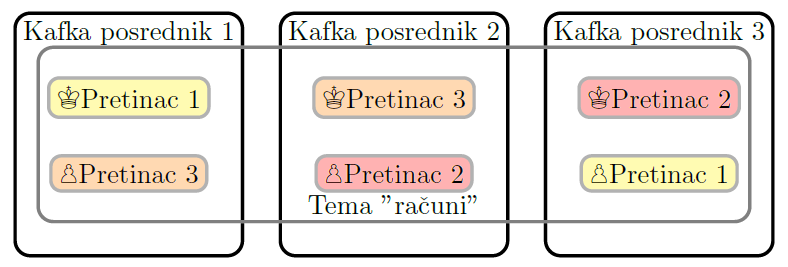
\includegraphics[width=0.8\textwidth]{KafkaPartitions.png}
    \caption{Pretinci vođe i pretinci sljedbenici}
    \label{fig:kafka-leader-follower}
\end{figure}

\ref{fig:kafka-leader-follower} prikazuje tri posrednika u grozdu. Tema "računi" je podijeljena na najveći mogući broj pretinaca: broj posrednika u grozdu. Kako se poruke ne bi izgubile zbog ispada posrednika svaki pretinac teme je umnožen jednom. Vođa žutog pretinca je nasumično posrednik jedan. Vođa crvenog pretinca će biti ili posrednik dva ili tri jer se vodstvo pretinaca mora jednoliko raspodijeliti. Ako vođa crvenog pretinca postane posrednik tri, onda će vođa narančastog pretinca postati posrednik dva. Pretinac pratitelji se ravnomjerno rasporede po posrednicima tako da pratitelji nikad nisu zajedno s vođom u istom posredniku.

Osim sto vođa pretinca je jedini posrednik koji može čitati ili pisati poruke iz pretinca, on se mora brinuti o pratiteljima. Vođa smatra da je pratitelj živ samo ako je prijavljen u Kafka grozd i ako ne zaostaje s čitanjem poruka iz pretinca vode. Ako zaostaje, vođa će pratitelja izbaciti iz skupa usklađenih pratitelja (ISR). Kada vođa primi poruke od objavljivača on će poruke zapisati u svoju particiju i čekat će potvrde pratitelja. Tek kada svi pratitelji pročitaju i zapišu poruke u svoj pretinac će vođa pretinca poslati potvrdu objavljivaču. Pretplatitelji mogu čitati samo one poruke koje su i vođa i pratitelji zapisali u svoje pretince.

Ako se posredniku koji je vođa pretinca dogodi ispad, nitko neće moći čitati ili pisati poruke u pretinac. Zato će pratitelji glasati tko će od pratitelja postati novi vođa pretinca. Samo pratitelji koji su u skupu ukradenih pratitelja mogu postati novi vođa. U iznimnom slučaju kada ne postoji usklađeni pratitelj neusklađeni pratitelj može postati novi vođa pretinca.

Posrednika, tema, pretinaca i umnoženih pretinaca je puno. Kako posrednici ne bi glasali za novog vođu pretinca za svaki pretinac zasebno jedan od posrednika je zadužen da bude nadglednik glasanja. Ako se dogodi ispad posrednika, nadglednik glasanja će ubrzati glasanje novog vođe pretinca.

\subsection{Pretplatnik}
Pretplatnik je korisnički program koji čita poruke iz teme. Svaki pretplatnik je član samo jedne skupine pretplatnika. Skupina pretplatnika može se sastojati od samo jednog člana. Skupina pretplatnika zajedno čita poruke iz teme. Svaki pretplatnik u skupini pretplatnika zadužen za čitanje poruka ima barem jedan pretinac iz kojeg jedino on može čitati poruke. Skupina pretplatnika može istovremeno napraviti najviše P čitanja ako je P broj pretinaca i u skupini pretplatnika je barem P članova. Poruke se mogu pročitati jedino iz pretinca vođe. Ako pretplatnik uputi zahtjev za čitanje pratitelju pretinca on će pretplatnika preusmjeriti na vođu pretinca.

Pretplatnik u zahtjevu za čitanje navodi odmak zadnje pročitane poruke i koliko poruka želi pročitati. Posrednik će dostaviti sve poruke od odmaka do tražene količine ili dok ne dođe do kraja pretinca. Odmak poruke je i jedinstvena oznaka poruke i mjesto u datoteci posrednika gdje se poruka nalazi. Posrednik ne pazi koje je poruke pretplatnik pročitao. Pretplatnik je zadužen za rukovanje odmakom. Odmak zadnje pročitane poruke pretplatnik šalje u posebnu temu posrednika. Ako se dogodi ispad pretplatnika, drugi pretplatnik će pročitati odmak iz teme i nastaviti s čitanjem poruka iz pretinca.

Posrednik će jednom pretplatniku po skupini pretplatnika dostaviti poruku barem jednom. Ako se dogodi ispad pretplatnika ista poruka se može dostaviti više puta. Ako je nedopustivo istu poruku pročitati više puta onda korisnik mora napraviti vlastiti algoritam ili koristiti transakcijskog pretplatnika. Pretplatnik čita poruke onim redoslijedom kojim su poruke zapisne u pretinac. Posrednici vremenski ne uređuju dostavu poruka iz svih pretinaca, ali su poruke vremenski uređene u svakom pretincu pojedinačno. Ako je potrebno vremenski urediti sve poruke u svim pretincima onda je potrebno razviti vlastiti algoritam ili napraviti temu sa samo jednim pretincem.

Više skupina pretplatnika može istovremeno citati poruke iz iste teme i pretinaca. Posrednik će odaslati istu poruku svim pretplaćenim pretplatnicima. Posrednici će skupu pretplatnika omogućiti čitanje poruka samo ako su svi pratitelji u skupu usklađenih pratitelja i vođa pretinca zapisali poruke u pretinac. Nakon što pretplatnik primi poruke on će u temi odmaka ažurirati odmak do kojeg je pročitao poruke.

Model povlačenja poruka pretplatnicima dopušta čitanje poruka brzinom koja njima odgovara. Model dopušta i učinkovito razašiljanje iste poruke na više pretplatnika. Ako pretplatnik želi ponovno pročitati poruku on samo treba poslati odmak pročitane poruke. Kako pretplatnik ne bi zaglavio u petlji ako u pretincu nema novim poruka on sebe može blokirati dok ne dođu nove poruke. Posrednik nikad ne zna kada su svi pretplatnici pročitali poruke i zato ih ne može obrisati nakon čitanja. Posrednici su zato napravljeni da s povećanjem nepročitanih poruka njihova učinkovitost ne opada. Posrednik će poruke izbrisati nakon zadanog vremena.

\section{Apache Pulsar}



\subsection{Objavljivac}
Objavljivac je korisnicki program koji salje poruke u temu. Poruke se nuzno sastoje od sadrzaja, oznake objavljivaca, jedinstvene oznake poruke i vremena objave. Poruke se mogu slati u skupini. Prije slanja, poruke se mogu sazeti. Tema moze biti podijeljena na pretince. Objavljivac moze usmjeriti poruke u odredeni pretinac. Poruke se mogu usmjeriti na jedan nasumicni pretinac, na tocno odredene pretince koristeci kljuc ili se mogu slati jednoliko na sve pretince. Objavljivaci ili cekaju potvrdu da je posrednik zapisao poruke ili nastave s radom i nakonadno provjeravaju jel su poruke primljene. 
SLIKA GROZDA


\subsection{Tema i pretplata}
Tema je imenovani tok poruka koji sluzi za prijenos poruka od objavljicava do pretplatnika. Svaka tema je izgradena kao poveznica. Svaka tema pripada prostoru imena. Prostor imena je upravna jednika kojom se mijenjaju postavke skupini tema. Svaki prostor imena pripada stanaru. Stanari pripadaju Pulsar grozdu. Moguce je napraviti bezmemorijske teme koje poruke cuvaju do slanja pretplatnicima ili ispada posrednika. Bezmemorijske teme objavljene poruke potiskuju prema pretplatnicima. Prednost bezmemorijskih tema je brzina. Kolicina neprocitanih poruka u temi ne utjece na protok poruka kroz temu. Poruka se brise iz teme kada svi pretplatnici procitaju poruku ili kada je poruka procitana i starija od zadane vrijednosti ili kada je neprocitana i starija od zadane vrijednosti. Tema se moze podijeliti na vise podtema zvanih pretinac. Pretinci su ravnomjerno raspodijeljeni po posrednicima. 
SLIKA RAPOSIJELE PRETINACA

Kako objavljivaci usmjeravaju dostavu poruka na pretince tako pretplatnici citaju poruka koristeci pretplate. Postoje tri vrste pretplata. Iskljuciva pretplata pravo citanja poruka daje samo jednom pretplatniku. Zajednicka pretplata jednoliko dostavlja poruke pretplatnicima. Sigurnosna pretplata pravo citanja daje samo jednom pretplatniku dok se pretplatniku ne dogodi ispad. Kada se dogodi ispad pomocni pretplatnik ce nastaviti citanje poruka od mjesta ispada. Zajednicka pretplata ne podrzava skupnu potvrdu dostave poruka niti pazi na vremensko uredenje dostave poruka.
SLIKA PRETPLATA



\subsection{Posrednik}
Posrednik je program bez stanja koji se sastoji od dva dijela. Prvi dio je posluzitelj s REST suceljem za upravljanje i pretrazivanje tema, a drugi dio je otpravnik za prijenos podataka. Umjesto da objavljivaci i pretplatnici izravno razgovaraju s posrednikom mogu se spojiti na zastupnika koji ce preusmjeriti njihove zahtjeve posrednicima.

Pulsar proces satoji se od barem jednog Pulsar grozda. Pulsar grozd sastoji se od barem jednog posrednika, Apache BookKeeper grozda i Apache ZooKeeper grozda. Pulsar grozdovi mogu umoziti poruke ako pripadaju istom procesu. Zadaca posrednik je posluziti poruke pretplatnicima iz upravljane knjige ili BookKeepera, dok je ZooKeeper zaduzen za cuvanje podata o grozdu. BookKeeper se brine o zapisivanju poruka.



\subsection{Upravljana knjiga}
BookKeeper grozd je raspodijeljeni zapisivac koji se sastoji od barem jednog zapisnicara. Zapisnicar zapisuju poruke koje mu posrednici posalju. Poruke se mogu umoziti i zapisati u vise knjiga odjednom. Svaka tema sastoji se od barem jedne knjige. Kapacitet poruka koji se moze zapisati moze se povecati dodavanjem zapisnicara. Zapisnicari mogu istovremeno citati i pisati poruke. 

Knjiga je struktura podatka u koju se poruke mogu dodati samo na kraj. Nakon sto se knjiga zatvori ona se jedino moze citati. Ako se zapisnicaru dogodi ispad, knjiga se zatvori. Kada se ispad otkloni zapisnicar ce ustanovit u kojem je stanju knjiga i ustanovljeno stanje poslati ostalim zapisnicarima u grozdu. 

Upravljana knjiga je skup BookKeeper knjiga u koju se upisuju poruke koje pripadaju jednoj temi. Makar se poruke mogu zapisati u samo jednu knjige vise BookKeeper knjiga olaksava brisanje i pisanje poruka. Upravljana knjiga sastoji se skupa tokova podata koji se zapisuju u knjigu s jednim pisacem i skupa pokazivaca koji prate koje poruke su pretplatnici procitali. Zapisivac prije pisanja poruke u upravljanu knjigu poruke zapisuje u dnevnik.


\subsection{Pretplatnik}
Pretplatnik je korisnicki program koji se pretplacuje na pretplatu teme. Postoje tri vrste pretplate. Svaka pretplata odreduje nacin na koji pretplatnik cita poruke. Pretplatnik moze ili biti blokiran dok posrednik ne dobije poruku ili nastaviti s radom i dobiti buducnostnicu kojom ce citati poruke. Pretplatnik moze pojedinacno ili skupno potvrditi poruke.

Ako korisnik nije zadovoljan izvedenim pretplatnikom on moze koristiti sucelje citaca. Sucelje citaca je biblioteka koja omogucuje rucno potvrdivanje poruka, ponovno citanje poruke i odbacivanje uvisestrucenih poruka.



\chapter{Unistenje visestrukih poruka}
Poruka se moze objaviti vise puta. Posrednik nece zapisati poruku koju zna da je vec zapisana.


\chapter{Korisnici}
Korisnik se pitati tko je zaduzen za temu. Nakon sto dobije adresu posrednika, spojt ce se na posrednika.

\chapter{Iznimke}
Koje f-nalnosti ne rade s kojima. TODO


\section{RabbitMQ}



\chapter{Postojeca rjesenja}

\chapter{Arhitektura rjesenja}

\chapter{Dizajn rjesenja}

\chapter{Izvedba rjesenja}

\chapter{Rezultati}

\chapter{Zaključak}
Zaključak.

\bibliography{literatura}
\bibliographystyle{fer}

\begin{sazetak}
Sažetak na hrvatskom jeziku.

\kljucnerijeci{Ključne riječi, odvojene zarezima.}
\end{sazetak}

\engtitle{Real-Time Health Monitoring in Distributed Data Stream Processing System}
\begin{abstract}
Abstract.

\keywords{Keywords.}
\end{abstract}

\end{document}
